\section{The Ranking Problem}\label{sec:ranking}
A ranking algorithm implements a function, which accepts a set of items and returns an ordered version of the set without modifying the items. The function is implemented taking into account certain preferences that determine the order of the items. In this way, the same collection of items could be ranked following different approaches, i.e. different order functions. 
Formally, a ranking algorithm implements a function of total order $f: X \rightarrow \Re$ such that for any $a, b \in X: f(a) \leq f(b) \leftrightarrow a \prec b$, where $\prec$ defines a binary relationship on the set $X$. Note that $\prec$ makes reference to the factor that guides the ranking strategy.

%TODO change image size and orientation
\begin{figure}[htbp!]
\begin{center}
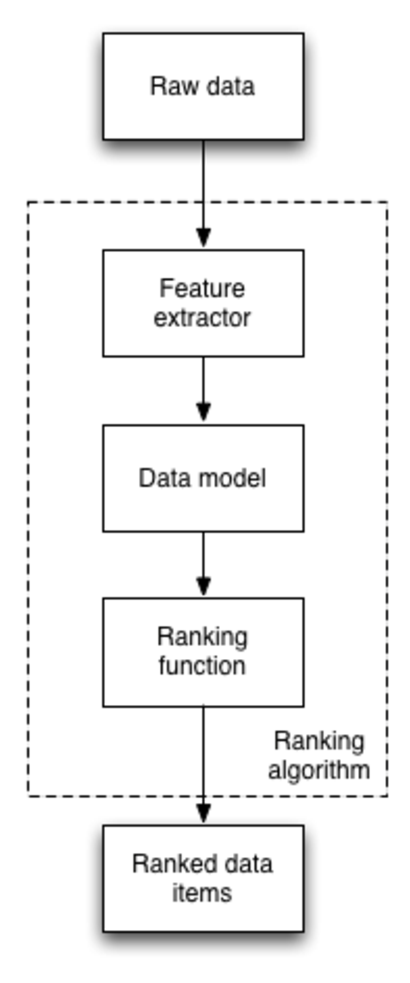
\includegraphics[width=0.35\textwidth]{figs/algo-arch.pdf}
\caption{{\bf Structure of a ranking algorithm}}
\label{fig:fig1}
\end{center}
\end{figure}

Figure \ref{fig:fig1} depicts the components that integrate the functionality of a ranking algorithm. The input to any ranking method is a bunch of raw data that needs to be inspected to get the relevant information out of it. This task is carried out by the feature extractor, which generates a data model that will be used for the ranking function described above to produce the ranked set of items. The feature extractor together with the data structures that allocate the data model and the ranking function compose the functional architecture of the ranking algorithm.



\subsection{Ranking on Structured Data}
Structured data: can be conceived as graphs\\
Ranking: traditionally, core IR problem, many techniques have been adopted to deal with structured data\\
Ranking over structured data: ranked list of results\\
Types of ranked results: entities, relations, subgraphs, entire datasets (graphs)\\
Evaluating ranked results: different metrics\\

\subsection{Ranking on Structured Data vs. Ranking on Unstructured Data}
Discuss differences\\
Say we focus on structured data\\

\subsection{Ranking vs. Matching}
Discuss differences\\
Say we focus on ranking\\


\subsection{Applications} 
%Optional / can be short but should provide good coverage of different application domains
Using information is directly related to the way in which it is presented and consumed. This means that without methodologies to exploit properly the data it can be very difficult to deal with the huge amount of information available. This function is carried out by ranking algorithms and a proof of its applicability is the different use cases where they can be deployed. In the following, we describe how ranking algorithms are used within semantic search engines, semantic browsers and interlinking approaches.

\subsubsection{Semantic Search Engines}
Like in the traditional hypertext Web, semantic search engines are used as the entry point to navigate the information burden. The architecture of these systems is built on top of a crawler which is responsible for automatically exploring the Web of Data to retrieve any piece of semantic information (RDF, RDFa, etc.). This stream of information fed by the crawler constitutes the knowledge base that will be used to resolve the users ́s queries. It is in this phase where ranking algorithms play their role, by means of manipulating the information in the knowledge base to calculate the relevance of results.
Table \ref{tab:tab} shows the existent semantic search engines and the correspondence with the underlying implemented ranking algorithm.

TODO table with sse

In the following, we describe the approach followed by each search engine.

\paragraph{Sindice}
Sindice (Tummarello, Delbru, Oren, 2007) is a lookup service built with the aim of enabling information retrieval over the resources of the semantic Web. Through crawling techniques, Sindice analyzes each source of data, i.e. RDF document or SPARQL endpoint, and extracts all the resources encountered. The information related to these resources is stored in an index that can be queried based on full-text search, URIs or inverse-functional properties (IFPs).

\paragraph{SemSearch}
SemSearch (Lei, Uren, Motta, 2006) is a keyword-based semantic search engine that tries to bring the power of the semantic Web to all kind of users regardless of their knowledge about semantic technologies while producing accurate results at the same time. It provides a Google- like interface which ranks the search results according to the degree of their proximity to the user query. The search engine takes two factors into consideration when ranking. One is the matching distance between each keyword and its semantic matches. The other is the number of keywords the search results satisfies. The matching strategy relies on simple string comparisons between the user keywords and the labels available in the RDF data sources. Authors justify this choice stating that “from the user point of view labels often catch the meaning of semantic entities in an understandable way”.

\paragraph{Swoogle}
Swoogle (Ding et al., 2004) was intended as a search engine for retrieving semantic Web documents. With this aim it is composed of a crawler than constantly checks the Web looking for new RDF or OWL documents containing any kind of semantic information. Once the documents are found, the system uses an index to store the information and facilitate the retrieval. In the same way than traditional search engines over HTML documents, Swoogle allows users to look for any term within the indexed documents. The way how results are returned to the user is determined by the OntologyRank algorithm.

\paragraph{Falcons}
Falcons (Cheng, \& Qu, 2009) is a keyword-based search engine supporting full-text queries related to data in the semantic Web. It works at entity level granularity, and so, for each entity it shows information about its types, possible labels and number of documents where it appears. The search engine is fully implemented relying on an index that stores textual information about each entity, as well as its relationships with other entities. Falcons applies the TF-IDF technique over the index to retrieve information about the entities and therefore about the ontologies where they appear.

\paragraph{Sig.ma}
(Tumarello et. al, 2009) describes the implementation of Sig.ma, an application that shows a possible interpretation of how the Web of Data functionality should look like. It combines large scale semantic web indexing, logic reasoning, data aggregation heuristics, ad hoc ontology consolidation, user interaction and refinement.
Sig.ma is built on top of Sindice, which means it follows the same ranking approach. More than a search engine, it has been designed with the aim of mashing up information, i.e., it gathers information from different sources and place it in a single interface to provide a richer experience to the user. Sig.ma can be considered as an extension to Sindice, which enables a refinement towards entity-oriented search.

\paragraph{SWSE}
The Semantic Web Search Engine (Hogan et. al, 2010) unlike other search engines works over Linked Open Data. It consists of crawling, data enhancing, indexing and a user interface for search, browsing and retrieval of information. It has been designed to deal with two main challenges: scalability to large amounts of data and tolerance to heterogeneous, noisy and conflicting data retrieved from different sources.
The search performed by the SWSE is focused on entities over instance data, in contrast to other approaches like Swoogle, which follows a document oriented search over ontologies. The underlying ranking strategy of SWSE relies on ReConRank, which means that it focuses on provenance of data to establish an order for results.

\paragraph{Watson}
Watson (d’Aquin et. al, 2007) is intended to be a gateway to access the content of the semantic Web. It provides keyword search facilities over semantic Web documents, but additionally provides search over entities. Authors establish that while following a traditional Web approach to retrieve information about ontologies is useful, it is not enough and must be complemented with specific techniques to exploit the semantics they model. In this way, approaches like OntologyRank that rely on the popularity of ontologies to establish the order of results are criticized, as they do not reflect the real quality of the information contained. In real scenarios, where the main aim of these systems is the reutilization, the quality of the ontology can be as important as its popularity. Therefore, Watson implements a ranking strategy similar to the one implemented by AKTiveRank, where the scores are calculated relying on exhaustive analysis to derive the quality of data.

\subsubsection{Semantic Browsers}
Browsers are the tool utilized by users to access the information on the Web. This means that the way how the information is presented to the users is a decisive factor for its consumption, because it determines the next steps for the user while the exploration. In the same way than traditional browsers explore the links between hypertext documents, semantic browsers intend to explore links between RDF data. Tabulator (Berners-Lee et al. 2006; Berners-Lee et al. 2008) and Marble (Becker \& Bizer, 2008) are two examples of semantic browsers that apply ranking methodologies to analyze the provenance of data at the same time that merging information from different data sources.

\subsubsection{Interlinking}
Interlinking can be defined as the process of creating new links between related entities in different RDF datasets for which there are not any link previously established. The final aim of interlinking is creating a network of related entities in order to facilitate its discovery and navigation of the Web of Data.
As introduced in (Bizer et. al, 2009), automatic and semi-automatic interlinking approaches rely on the computation of similarities between entities, mostly guided by related work on record linkage, duplicate detection in databases and ontology matching. However, what is not directly mentioned is that ranking algorithms can complement interlinking methods by providing previous analysis of data. Statistics about entities can give information about the truthfulness of concepts as stated in (Bizer \& Cyganiak, 2009). For example, if a concept representing the city of Barcelona is pointed from different sources where properties make reference to this city, it means there is a chance that this concept really represents the city of Barcelona. In this way, the number of links targeting the same concept could be used as an indicator of the veracity of such concept when referring to an entity of the real world.